% Chapter Template
\chapter{Results and discussion} % Main chapter title
\label{Results} % for referencing this chapter elsewhere, use \ref{ChapterX}
%\lhead{Results and discussion} % this is for the header on each page - perhaps a shortened title
\fancyhead[RO,LE]{Results and discussion}
\fancyfoot[C]{\thepage}

The following chapter summarizes the methods and insights of the four manuscripts that can be found in the appendix of this thesis.

\aref{SuppPub_NSL} corresponds to Lam, Mühlpfordt, Vaquerizas et al. (2012) \citep{Lam2012} where we examined the \textit{Drosophila} ChIP-seq profiles of four members of the NSL complex (NSL1, NSL3, MCRS2, MBD-R2; generated by Sunil Raja and Kin Chung Lam) and ChIP-seq data for Pol~II from S2 cells depleted of either NSL1 or NSL3 (experiments by Kin Chung Lam).

\aref{SuppPub_MSL} corresponds to Chelmicki, Dündar et al. (2014) \citep{Chelmicki2014} for which Tomasz Chelmicki generated ChIP-seq data of MOF, MSL1, MSL2, NSL3, MCRS1 in mouse embryonic stem cells and neuronal progenitor cells. Matthew Turley and Tasneem Khanam generated transcriptome data for cells depleted of individual factors.

\aref{SuppPub_deepTools} corresponds to Ramirez, Dündar et al. (2014) \citep{Ramirez2014}, the publication of a software suite for quality control, normalization and visualization of high-throughput sequencing data.

\aref{SuppPub_MSL1} corresponds to the submitted manuscript by Chlamydas et al. that focuses on the general role of fly and mammalian MSL1 at promoters and makes use of the ChIP-seq profiles of MSL1 in \textit{D.~virilis}, \textit{D.~melanogaster} and mouse.
%------------------------------------------------------------------
%	SECTION 
%------------------------------------------------------------------
\section{Setting up a ChIP-seq analysis workflow}
One of the main goals of my PhD studies was to identify pitfalls and optimized methods of ChIP-seq analyses whose basics had been established in our group by Sarah Diehl and Thomas Manke. In short, there were three main insights:
\begin{itemize}[topsep=0pt]
\item Understanding biases of the data is crucial for the analysis as well as for improved experimental procedures.
\item Standardized bioinformatic workflows must always be coupled to manual inspections and iterative optimization depending on the quality and nature of the data set and the questions to be answered.
\item Any software for analysis of high-throughput sequencing data must be inherently designed with some flexibility as the applications, sequencing platforms, file formats, data types and statistical models are constantly evolving.
\end{itemize}
%
%--------------------------------------
%%% Figure ChIP-seq workflow
\begin{figure}
 \begin{minipage}[c]{0.6\textwidth}
   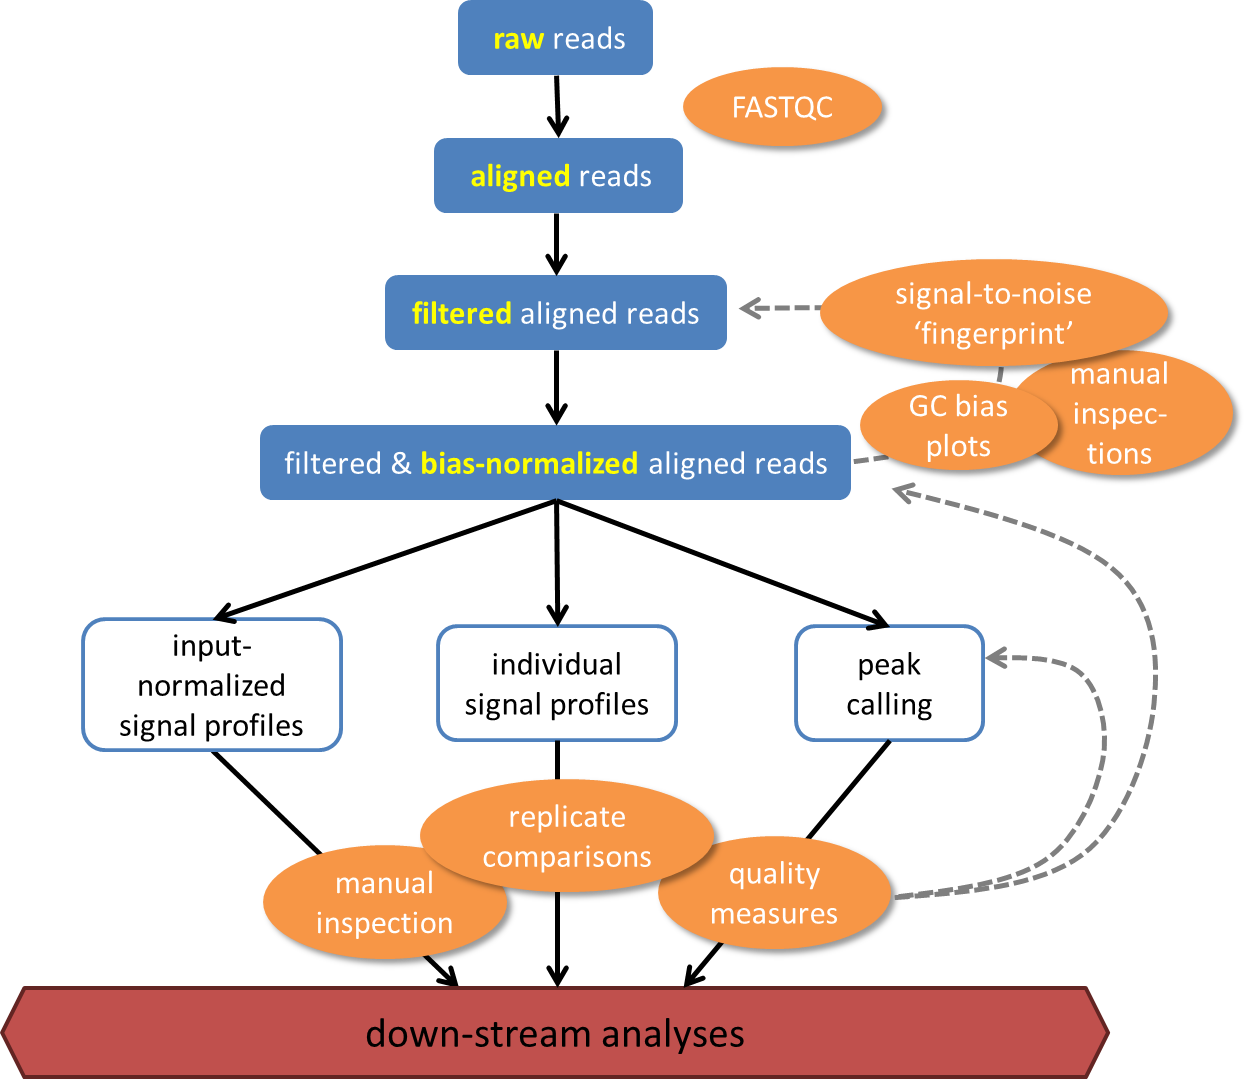
\includegraphics[width=\textwidth]{Figures/workflowChIP-seq.png}
 \end{minipage}\hfill
 \begin{minipage}[c]{0.35\textwidth}
	\begin{footnotesize}
   \caption[General bioinformatics workflow for ChIP-seq analyses.]{\textsf{Schematic of the general bioinformatics workflow for ChIP-seq analyses.
	Orange circles depict quality controls, boxes with solid blue fill indicate read-based files (FASTQ and SAM/BAM, for file name explanations see the glossary of \aref{SuppPub_deepTools}), white boxes indicate files based on genomic intervals. The in\-for\-ma\-tion of the various quality checks help to adjust all steps to match the samples' properties and the ultimate biological questions to be answered.
}}
\label{fig:workflow}
\end{footnotesize}
 \end{minipage}
\end{figure}
%---------------------------------
%
%%\begin{landscape}
\begin{singlespacing}
\begin{small}
%\setlength{\extrarowheight}{15pt} % this doesn't work to control the vertical space
\vspace*{-1em}
\begin{longtable}{>{\textsf\bgroup\raggedleft\arraybackslash}p{2.7cm}<{\egroup} >{\textsf\bgroup}p{4.5cm}<{\egroup} >{\textsf\bgroup}p{4.2cm}<{\egroup}>{\textsf\bgroup}p{2.3cm}<{\egroup}} % defining the columns - these must match the widths defined for the mini pages down below!
\caption[Bioinformatic tools used for analyses presented here.]{\textsf{Bioinformatic tools used for analyses presented here (alphabetical order; if available, I indicated the versions of the tools that I used). For explanations of the file formats mentioned here, please see the glossary within the supplement of \aref{SuppPub_deepTools}.}} \\ % the \\ is important! see http://tex.stackexchange.com/questions/103698/extra-alignment-tab-with-longtable
%%%%%%%%%%%%%%%
% table title
\textbf{Name} & \textbf{Application} & \textbf{Website} & \textbf{Reference}
\tabularnewline \hline
\endfirsthead % indicates that the lines above appear as head of the table on the first page
\multicolumn{4}{c}%
{\tablename\ \thetable\ -- \textit{Continued from previous page}} \\[1ex]
\textbf{Name} & \textbf{Application} & \textbf{Website} & \textbf{Reference}
\tabularnewline \toprule %\tabularnewline [1ex]
\endhead % Line(s) to appear at top of every page (except first)
\multicolumn{4}{r}{\textit{Continued on next page}} \\
\endfoot % Last line(s) to appear at the bottom of every page (except last)
\endlastfoot
%%%%%%%%%%%%%%%%%%%
%% first row
%-----------------------
\toprule %\\ [4ex]
 \begin{minipage}{2.7cm}
				\textbf{bedtools} \\
					(2.10. to 2.17)
				\end{minipage}
			&	 \begin{minipage}{4.5cm}
				working with genomic intervals, e.g. intersecting two files with different peak regions
			\end{minipage} 
			&  \begin{minipage}{4.2cm}
			\url{http://bedtools.readthedocs.org/en/latest/}
			\end{minipage} 
			&  \begin{minipage}{2.3cm}
					\raggedright \citet{Quinlan2010}
				\end{minipage} 
%\\ [4ex] \hline \\ [1ex]
\tabularnewline \midrule
%---------------------------
 \begin{minipage}{2.7cm}
				\textbf{bowtie} \\
					bowtie-1.0.0\\(Appendix \ref{SuppPub_NSL}),\\
					bowtie2-2.2.2\\(Appendix \ref{SuppPub_MSL}) %\\ [2ex]
			\end{minipage} 
			&  \begin{minipage}{4.5cm}
			alignment of reads to the reference genome
				\end{minipage} 
				&  \begin{minipage}{4.2cm}
				\url{http://bowtie-bio.sourceforge.net/index.shtml}
				\end{minipage} 
				&  \begin{minipage}{2.3cm}
				Langmead and\\
				Salzberg \citep{Langmead2012}
			\end{minipage} 
%\\ [4ex] \hline \\ [1ex]
\tabularnewline \midrule
%-----------------------
 \begin{minipage}{2.7cm}
				\textbf{ChIPEnrich}
			\end{minipage} 
			&  \begin{minipage}{4.5cm}
					gene ontology enrichments for target genes identified by ChIP-seq
			\end{minipage} 
			&  \begin{minipage}{4.2cm}
					\url{http://sartorlab.ccmb.med.umich.edu/chip-enrich}
			\end{minipage} 
			&  \begin{minipage}{2.3cm}
				\citet{Welch2014}
			\end{minipage} 
%\\ [4ex] \hline \\ [1ex]
\tabularnewline \midrule
%-----------------------------
 \begin{minipage}{2.7cm}
		\textbf{DAVID}
\end{minipage} 
			&  \begin{minipage}{4.5cm}
				gene identifier mapping and gene ontology term enrichment analyses
			\end{minipage} 
			&  \begin{minipage}{4.2cm}
				\url{http://david.abcc.ncifcrf.gov/}
			\end{minipage} 
				&  \begin{minipage}{2.3cm}
				\citet{Huang2009}
			\end{minipage} 
%\\ [4ex] \hline \\ [1ex]
\tabularnewline \midrule
%-----------------------------
 \begin{minipage}{2.7cm}
					\textbf{deepTools} \\
					(up to 1.5.7) %\\ [2ex]
			\end{minipage} 
			&  \begin{minipage}{4.5cm}
				quality controls of BAM files, normalizations, coverage file generation, visualizations with heatmaps and summary plots %\\ [2ex]
			\end{minipage} 
			&  \begin{minipage}{4.2cm}
				\url{http://deeptools.github.io/} %\\ [2ex]
			\end{minipage} 
				&  \begin{minipage}{2.3cm}
		\raggedright Ramirez, Dündar et al. \citep{Ramirez2014} %\\ [2ex]
			\end{minipage} 
%\\ [4ex] \hline \\ [1ex]
\tabularnewline \midrule
%-----------------------------
 \begin{minipage}{2.7cm}
					\textbf{DESeq}\\
					(1.10.1)
				\end{minipage} 
			&  \begin{minipage}{4.5cm}
				calculating normalized fold change values for Pol~II ChIP-seq data set \citep{EBIroutine}
			\end{minipage} 	
			&  \begin{minipage}{4.2cm}
				\url{http://www-huber.embl.de/users/anders/DESeq/}
			\end{minipage}
				& 
				\begin{minipage}{2.3cm}
		\citet{Anders2010}
			\end{minipage} 
%\\ [4ex] \hline \\ [1ex]
\tabularnewline \midrule
%---------------------------
 \begin{minipage}{2.7cm}
				\textbf{fastqc}
				\end{minipage}
			&  \begin{minipage}{4.5cm}
				quality control of FASTQ files
			\end{minipage} 
			&  \begin{minipage}{4.2cm}
				\url{http://www.bioinformatics.babraham.ac.uk/projects/fastqc/}
			\end{minipage} 
			&  not available
%\\ [4ex] \hline \\ [1ex]
\tabularnewline \midrule
%-----------------------------
 \begin{minipage}{2.7cm}
				\textbf{Galaxy} %%\\ [2ex]
				\end{minipage} 
			&  \begin{minipage}{4.5cm}
				vast collection of tools for manifold tasks including working with genomic intervals, joining of lists, motif search etc. %\\ [2ex]
			\end{minipage} 
			&  \begin{minipage}{4.2cm}
				in-house installation %%\\ [2ex]
			\end{minipage} 
					&  \begin{minipage}{2.3cm}
		\citet{Goecks2010} %%\\ [2ex]
			\end{minipage} 
%\\ [4ex] \hline \\ [1ex]
\tabularnewline \midrule
%-----------------------------
 \begin{minipage}{2.7cm}
					\textbf{ggplot2}\\
					(0.9.3.1)
			\end{minipage} 
			&  \begin{minipage}{4.5cm}
				R package for highly customizable plots (e.g. boxplots, x-y plots, bar charts etc.)
			\end{minipage} 
			&  \begin{minipage}{4.2cm}
				\url{http://ggplot2.org/}
			\end{minipage} 
			&  \begin{minipage}{2.3cm}
		\citet{ggplot2}
			\end{minipage} 
%\\ [4ex] \hline \\ [1ex]
\tabularnewline \midrule
%-----------------------------
 \begin{minipage}{2.7cm}
					\textbf{GREAT}\\
					(2.0)
				\end{minipage} 
			&  \begin{minipage}{4.5cm}
				web-based tool for target gene prediction
			\end{minipage} 
			&  \begin{minipage}{4.2cm}
				\url{http://bejerano.stanford.edu/great/public/html/}
			\end{minipage} 
				&  \begin{minipage}{2.3cm}
		\citet{McLean2010}
			\end{minipage} 
%\\ [4ex] \hline \\ [1ex]
\tabularnewline \midrule
%----------------------------
 \begin{minipage}{2.7cm}
					\textbf{Integrative\\Genomics\\Viewer}\\
					(up to 2.3.32) %\\ [2ex]
			\end{minipage} 
			& 	\begin{minipage}{4.5cm}
				genome browser for visualization of BAM, BED, bigWig and bedGraph files %\\ [2ex]
			\end{minipage} 
			&  \begin{minipage}{4.2cm}
				\url{http://www.broadinstitute.org/igv/} %\\ [2ex]
			\end{minipage} 
				&  \begin{minipage}{2.3cm}
		\citet{Thorvaldsdottir2013} %\\ [2ex]
			\end{minipage} 
%\\ [4ex] \hline \\ [1ex]
\tabularnewline \midrule
%-----------------------------
 \begin{minipage}{2.7cm}
					\textbf{liftover}\\
					(2013)
			\end{minipage} 
			&  \begin{minipage}{4.5cm}
				conversion of sequence coordinates from mm8 assembly to mm9
			\end{minipage} 
			&  \begin{minipage}{4.2cm}
				\url{https://genome.ucsc.edu/cgi-bin/hgLiftOver}
			\end{minipage} 
				&  not available
%\\ [4ex] \hline \\ [1ex]
\tabularnewline \midrule
%-----------------------------
 \begin{minipage}{2.7cm}
				\textbf{MACS}\\
					(1.4.2)
				\end{minipage}
			&	 \begin{minipage}{4.5cm}
				identification of significantly enriched ChIP-seq regions
			\end{minipage} 
			&  \begin{minipage}{4.2cm}
				\url{http://liulab.dfci.harvard.edu/MACS/}
			\end{minipage} 
				&  \begin{minipage}{2.3cm}
		\citet{Zhang2008}
			\end{minipage} 
%\\ [4ex] \hline \\ [1ex]
\tabularnewline \midrule
%-----------------------------
 \begin{minipage}{2.7cm}
				\textbf{MEME}\\
					(4.9.0)
				\end{minipage} 
			&  \begin{minipage}{4.5cm}
				\textit{de novo} DNA motif identification
			\end{minipage}
			&  \begin{minipage}{4.2cm}
				\url{http://meme.nbcr.net/meme/}
			\end{minipage} 
					&  \begin{minipage}{2.3cm}
		\raggedright  \citet{Bailey1994, Machanick2011}
			\end{minipage} 
%\\ [4ex] \hline \\ [1ex]
\tabularnewline \midrule
%-----------------------------
\begin{minipage}{2.7cm}
				\textbf{PeakSplitter}\\
					(1.0)
				\end{minipage} 
			&  \begin{minipage}{4.5cm}
				splitting peak regions predicted by MACS into separate regions based on local minima detection
			\end{minipage} 
			&  \begin{minipage}{4.2cm}
				\url{http://www.ebi.ac.uk/research/bertone/software}
			\end{minipage} 
			&  \begin{minipage}{2.3cm}
		\citet{Salmon2010}
			\end{minipage} 
%\\ [4ex] \hline \\ [1ex]
\tabularnewline \midrule
%-----------------------------
 \begin{minipage}{2.7cm}
					\textbf{samtools}\\
					(0.1.19)
			\end{minipage} 
			&	 \begin{minipage}{4.5cm}
				SAM and BAM file handling (indexing, number of mapped/unmapped and uniquely reads etc.)
			\end{minipage} 
			&  \begin{minipage}{4.2cm}
				\url{http://samtools.sourceforge.net/}
			\end{minipage} 
				&  \begin{minipage}{2.3cm}
		\citet{Li2009}
			\end{minipage} 
%\\ [4ex] \hline \\ [1ex]
\tabularnewline \midrule
%-----------------------------
 \begin{minipage}{2.7cm}
					\textbf{TRAP}\\
					(Annotate v3.04)
				\end{minipage} 
			&  \begin{minipage}{4.5cm}
				transcription factor binding affinity calculation
			\end{minipage} 
			&  \begin{minipage}{4.2cm}
				\url{http://trap.molgen.mpg.de/PASTAA.htm}
			\end{minipage} 
				&  \begin{minipage}{2.3cm}
		\citet{Roider2007}
			\end{minipage} 
%\\ [4ex] \hline \\ [1ex]
\tabularnewline \midrule
%-----------------------------
 \begin{minipage}{2.7cm}
				\textbf{UCSC tools} \\
					(2013)
				\end{minipage} 
			&  \begin{minipage}{4.5cm}
				format conversion (bedGraph to bigWig)
			\end{minipage} 
			&  \begin{minipage}{4.2cm}
				\url{http://www.broadinstitute.org/igv/}
			\end{minipage} 
					&  \begin{minipage}{2.3cm}
		\citet{Kent2010}
			\end{minipage} 
%\\ [4ex] \hline \\ [1ex]
\tabularnewline \midrule
%-----------------------------
 \begin{minipage}{2.7cm}
				\textbf{Venny}\\
					(2007)
				\end{minipage} 
			& 	\begin{minipage}{4.5cm}
				generation of Venn diagrams
			\end{minipage} 
			&  \begin{minipage}{4.2cm}
				\url{http://bioinfogp.cnb.csic.es/tools/venny/}
			\end{minipage} 
			&  not available
%\\ [4ex] \hline \\ [1ex]
\tabularnewline \bottomrule
%-----------------------------
\label{tab:tools}
\end{longtable}
\end{small}
\end{singlespacing}
%\end{landscape}

%
My current workflow for ChIP-seq analysis is depicted in \fref{fig:workflow}. It depends heavily on deepTools, a software package that was developed in collaboration with Fidel Ramírez \citep{Ramirez2014} (\tref{tab:tools}). The workflow begins with the sequencing information stored as DNA reads in FASTQ format (for details on the file formats, see the glossary within the supplement of \aref{SuppPub_deepTools}). The reads are aligned using bowtie2 \citep{Langmead2012} with default parameters. I usually discard unmapped, non-uniquely aligned, duplicated and low-quality reads, as well as those mapped to unassembled and mitochondrial chromosomes, to major satellites and other regions with obvious copy number variations. These rather aggressive filtering steps will probably yield non-optimal results for data sets with expected enrichments along repetitive regions and would have to be adjusted accordingly. However, particularly the removal of regions that consistently accumulated extremely high read numbers in both ChIP and input samples, improved the accuracy of scaling factor calculations and peak calling for the data sets that I analyzed (in line, the ENCODE consortium recently published a list of regions whose exclusion from the analysis improved data processing \citep{Blacklists, Carroll2014}). The optimization of the filtering steps was based on various quality controls, e.g. the assessment of the ChIP strength using the method proposed by \citet{Diaz2012}, manual inspections and GC bias checks.
%
\subsection{GC bias normalization}
%%% Figure GC bias
\begin{figure}[tb]
\centering
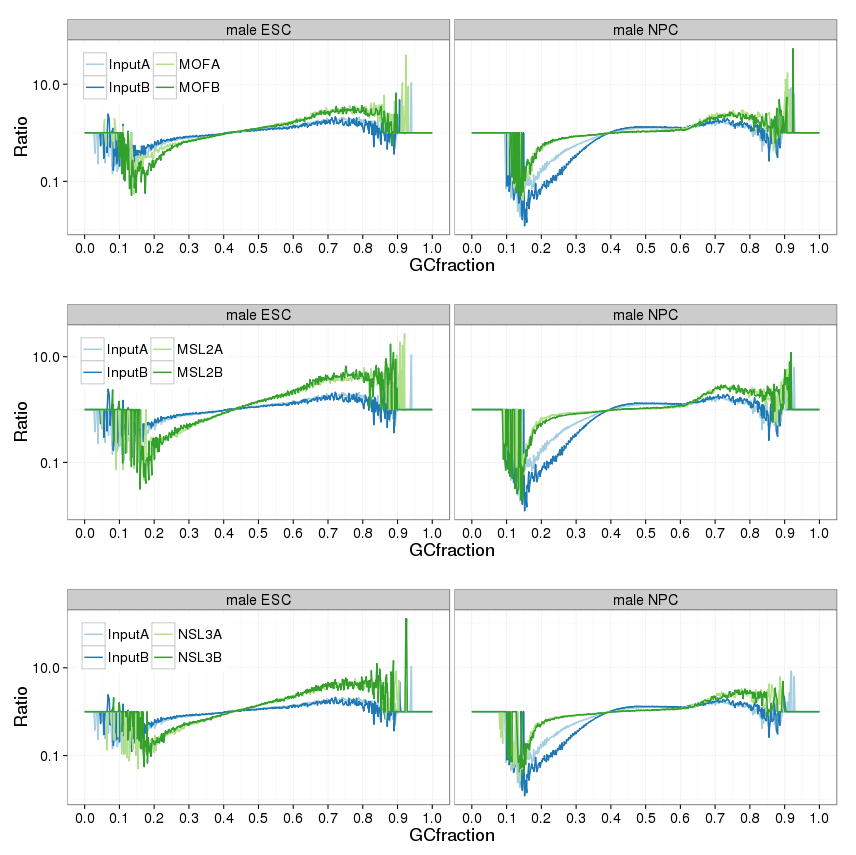
\includegraphics[width=0.9\textwidth]{Figures/ratios_mlES_mlNPC_MOF-NSL3-MSL2.png}
\begin{footnotesize}
\caption[Ratios of observed over expected read counts per GC content bin in ChIP-seq samples from murine embryonic stem cells and neuronal progenitor cells.]{\textsf{Different ratios of observed over expected read counts per GC content bin in ChIP-seq samples from embryonic stem cells (ESC) and neuronal progenitor cells (NPC). Green lines show the ratios for ChIP-seq samples (two replicates each), inputs are shown in blue, note the log scale. Ratios below zero indicate underrepresented regions, ratios above zero overrepresentation. The vast majority of the mouse genome will be covered by regions with 35-60\% GC content, thus any bias between 0.35-0.60 (y-axis) should be paid attention to. The sequencing libraries of the ESC samples were prepared with standard Illumina polymerase, while NPC samples were done with fewer PCR cycles and the HighFidelity Polymerase from New England Biolabs. The lack of AT-rich regions in the input samples is most likely due to other experimental steps than PCR (\tref{tab:biases}). The values underlying the images were calculated with the \texttt{computeGCBias} tool of deepTools \citep{Ramirez2014}.
}}
\label{fig:GCbias}
\end{footnotesize}
\end{figure}
%---------------------------------
The most prevalent and possibly distorting bias that is introduced by Illumina’s PCR-based library preparation and sequencing method (\tref{tab:sequencing}) is the overrepresentation of GC-rich regions. \citet{Benjamini2012} demonstrated that even if the input is handled like the ChIP sample during the experiments, it will unlikely suffice to correct for abundant GC bias because the extent and the regions that are overamplified were shown to be specific for each library preparation. In the light of their insights, we examined the GC bias of the mouse ChIP-seq samples that later on were the basis for Chelmicki, Dündar et al \citep{Chelmicki2014}. As shown in \fref{fig:GCbias}, the different samples indeed had distinct GC bias profiles and the observation that the bias was dramatically reduced when an optimized DNA polymerase and fewer PCR cycles were used (second column of \fref{fig:GCbias}) confirmed the claim of \citet{Benjamini2012} that the DNA amplification steps were the major cause of GC bias. Nevertheless, we identified additional issues that need to be taken into account before adjusting the observed read distributions: 
%
\begin{enumerate}[topsep=0pt]
\item ChIP-seq samples with strong enrichments at mammalian (typically GC-rich) promoters will have a biologically meaningful overrepresentation of GC-regions. This can, for example, be seen in the NPC ChIP-seq samples in \fref{fig:GCbias} where regions with more than 60\% GC content are overrepresented. This is due to the preferred binding of the investigated proteins to CpG-rich promoters.
\item In contrast to the claim that the GC bias should be library-specific, replicates of the same experiment showed very similar GC profiles, indicating a dominant ChIP- (and input-) specific effect.
\item The calculation of the expected read distributions is based on the available genome assembly whose quality might influence the outcome, especially if regions with strong sequence composition biases are not included in the assembly.
\end{enumerate}
%
We addressed the first two issues by a)~excluding unmappable as well as significantly enriched regions from the read distribution calculation and b)~in the case of the non-optimal (standard Illumina) library preparation, we decided to manually scale the input samples to each ChIP-seq so that the input samples reflected the ChIP-seq-specific GC bias rather than eliminating reads from GC-rich regions.

Perhaps the most important insight from these studies was the fact that optimized ChIP and sequencing protocols that were eventually enforced by our in-house sequencing facility almost completely eliminated GC biases. Individual samples at times still indicate the need for computational correction that should, however, be done with care and full knowledge of possible new artifacts that might be introduced such as the loss of enrichments in GC-rich regions\footnote{GC bias correction is applied on the files containing the aligned reads: reads in overrepresented regions are removed randomly, while underrepresented region will obtain artificially duplicated reads.}. In contrast to the BEADS package \citep{Cheung2011} that offers one standardized GC bias correction workflow, deepTools calculates and normalizes the read distributions using two separate tools (\texttt{computeGCbias} and \texttt{correctGCbias}, \aref{SuppPub_deepTools}), so that users can explore the expected and observed values first and thereupon decide which normalization strategy might best suit their data set. 
%
\subsubsection{Normalization for sequencing depth and input control}
Once the read alignments have been thoroughly checked and possibly normalized, the next steps lay the foundation for the majority of ChIP-seq downstream analyses that are typically not dependent on the DNA sequence of each read, but instead rely on summaries of the number of overlapping reads at each given locus in the genome (\fref{fig:readsCoverages} and white boxes in \fref{fig:workflow}).
I will usually first generate coverage profiles for each sample individually, normalizing for sequencing depth only:
\begin{center}
$normalized\:bin\:coverage = \frac{observed\:bin\:coverage \times e\!f\!\!f\!ective\:genome\:size}{mapped\:reads \times f\!ragment\:length}$\\
\end{center}
These profiles are useful to confirm that the input-normalized ChIP-seq signals and the peak calling results (see below) match the patterns seen in the simple coverages.

For input normalization, both input and ChIP must be made comparable first before calculating the ChIP enrichments ($log_2\frac{ChIP}{input}$) for each consecutive genomic bin. If the output of deepTools’ \texttt{bamFingerprint} \citep{Diaz2012} indicates a clear ChIP-seq signal compared to the input \citep{bamFingerprint}, I tend to use the signal extraction scaling (SES) proposed by \citet{Diaz2012}. SES is based on the assumption that the ChIP-seq sample contains both background and immunoprecipitated DNA and that the scaling factor for sequencing depth adjustment should be based on the background signal only. In a plot depicting the cumulative percentage of reads, the input should show a linear increase as each genome region should contain a similar fraction of reads (see the image of \texttt{bamFingerprint} in the supplemental material of \aref{SuppPub_deepTools}). ChIP-seq data, however, will contain a significant fraction of regions with consistently very few reads (= background) and a relatively small number of regions with exceedingly large read numbers (= immunoprecipitated DNA). The SES factor is the ratio of ChIP-seq over input reads at the point where the percentage of input reads maximally exceeds the percentage of ChIP-seq reads \citep{Diaz2012}.
If the separation between background and enrichment signal is not possible, the total number of reads of the less deeply sequenced sample ($n$) can be used to adjust the sequencing depths:
\begin{center}
$ scale\:f\!actor = \frac{n}{mapped\:reads}$ \\
\end{center}
All above described methods are implemented in \texttt{bamCoverage} and \texttt{bamCompare} of the deepTools suite (\aref{SuppPub_deepTools}).
%
\subsection{Peak calling}
%
As described in the introduction, the identification of significantly enriched genome regions is central to the majority of ChIP-seq analysis \citep{Bailey2013} (\fref{fig:dataProcessing}). I chose different peak calling strategies to meet the distinct challenges of each analyzed data set (summarized in \tref{tab:peakCallingStrategies}). All approaches rely on stringent filtering after obtaining the initial lists of significantly enriched regions, but only the Pol~II ChIP-seq and the mouse data set allowed for additional selection of peaks found in two replicates. 
%
%\begin{landscape}
\begin{singlespacing}
\begin{small}
\begin{longtable}{>{\textsf\bgroup}p{3.5cm}<{\egroup} >{\textsf\bgroup}p{4cm}<{\egroup} >{\textsf\bgroup}p{8cm}<{\egroup}>{\textsf\bgroup}p{6.5cm}<{\egroup}} % defining the columns - these must match the widths defined for the mini pages down below!
\caption[Peak calling strategies adjusted for the different sample characteristics.]{\textsf{Peak calling strategies adjusted for the different ChIP-seq sample characteristics.}} \\ % the \\ is important! 
%%%%%%%%%%%%%%%
% table title
\textbf{ChIP-seq sample} & \textbf{Issues} & \textbf{Strategy} &  % 
\tabularnewline \hline
\endfirsthead % indicates that the lines above appear as head of the table on the first page
\multicolumn{4}{c} 
{\tablename\ \thetable\ -- \textit{Continued from previous page}} \\
\textbf{ChIP-seq samples} & \textbf{Issues} & \textbf{Strategy} &  % 
\tabularnewline \toprule \tabularnewline [1ex]
\endhead % Line(s) to appear at top of every page (except first)
\hline \multicolumn{4}{r}{\textit{Continued on next page}} \\ %
\endfoot % Last line(s) to appear at the bottom of every page (except last)
\endlastfoot
%%%%%%%%%%%%%%%%%%%
%%% let's start the table content; each column (often) gets its own minipage which enables itemized lists etc.
%%%%%%%%%%%%%%%%%%%
%% first row
%-----------------------
\toprule
\begin{minipage}[c]{3.5cm}
NSL1, NSL3,\\MCRS2, MBD-R2 in\\\textit{D.~melanogaster}
\end{minipage}
			& \begin{minipage}[c]{4cm}
			peak regions often contained more than one local maximum due to the gene-dense nature of the \textit{Drosophila} genome
			\end{minipage}
				& \begin{minipage}[c]{8cm}
				\begin{enumerate}[noitemsep, leftmargin=*]
					\item peak calling with MACS 1.4.2 with default parameters \citep{Feng2012}
					\item peaks with FDR $\leq$ 5\%
					\item identification of smaller \textsl{subpeaks} with PeakSplitter \citep{Salmon2010}
				\end{enumerate}
				\end{minipage}
					& \begin{minipage}[c]{6.5cm}
					\parbox[c]{1em}{
						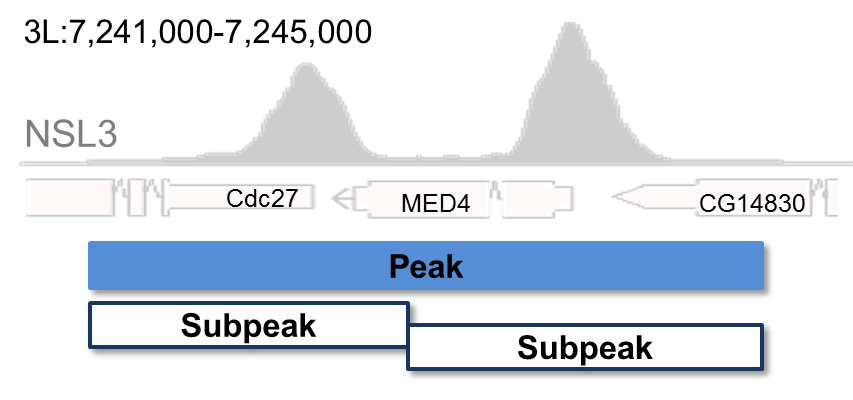
\includegraphics[width=6.5cm,trim=2 2 2 2,clip]{Figures/PeakCalling_Dmel}}
				\end{minipage} 
%\\ [2ex]  \hline \\ [1ex]
\tabularnewline \midrule
%-----------------------
\begin{minipage}[c]{3.5cm}
Pol~II in\\\textit{D.~melanogaster} cells\\(depleted of NSL1 or NSL3)
\end{minipage}
	& \begin{minipage}[c]{4cm}
	the mixed signal of Pol~II (localized, TF-like enrichments around TSS, broad, shallow enrichments along gene bodies) was not well captured by MACS
		\end{minipage}
		& \begin{minipage}[c]{8cm}
\vskip 6pt
				\begin{enumerate}[noitemsep, leftmargin=*]
					\item a symmetric null distribution was fitted to regions with negative enrichments, i.e. where the input signal exceeded the ChIP signal \citep{EBIroutine} (black line)
					\item genomic bins that deviated from the expectation (compare the blue with the black line) were determined as significantly enriched (threshold: q-value $\leq$ 0.05) \\ [2ex]
				\end{enumerate}
\vskip 4pt
			\end{minipage}
				& \begin{minipage}[c]{6.5cm}
						\parbox[c]{1em}{
						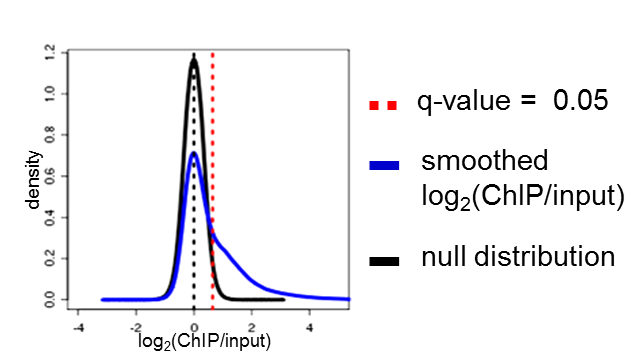
\includegraphics[width=6.5cm,trim=4 4 4 4,clip]{Figures/PeakCalling_PolII}}
					\end{minipage}
%\\ [2ex] \hline \\ [1ex]
\tabularnewline \midrule
%-----------------------
\begin{minipage}[c]{3.5cm}
MOF, MSL1, MSL2,\\NSL3, MCRS1 in\\ mouse ESCs and NPCs
\end{minipage}
	& \begin{minipage}[c]{4cm}
	non-optimal signal-noise ratios, GC bias
		\end{minipage}
		& \begin{minipage}[c]{8cm}
\vskip 6pt
				\begin{enumerate}[noitemsep, leftmargin=*]
                    \item in ESCs: adjustment of the GC bias in the input sample to match each ChIP-seq sample's GC bias
					\item peak calling with MACS 1.4.2 with default parameters \citep{Feng2012} for each ChIP-seq replicate (blue boxes) and the merged file (red box)
					\item only peaks that were present in both replicates and met the FDR threshold of $\leq$ 1\% were used \\ [2ex]
				\end{enumerate}
\vskip 4pt
			\end{minipage}
				& \begin{minipage}[c]{6.5cm}
\vskip 6pt
						\parbox[c]{1em}{
						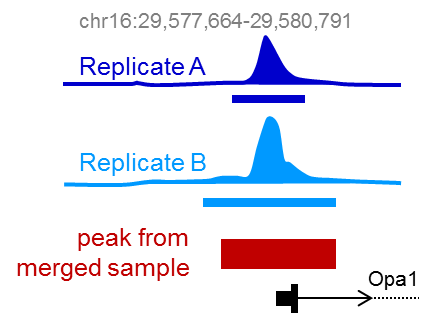
\includegraphics[width=5.5cm,trim=4 4 4 4,clip]{Figures/PeakCalling_Mm}} 
\vskip 4pt
					\end{minipage}
%\\ [2ex] \hline \\ [1ex]
%-----------------------
\tabularnewline \bottomrule
\label{tab:peakCallingStrategies}
\end{longtable}
\end{small}
\end{singlespacing}
\end{landscape}
 % moved to appendix
%
\subsection{Exemplary downstream analyses}
%---------------------------------
%%% Figure Summary plots and heatmaps of NSL, MSL in D.mel 
\begin{figure}[tb]
\centering
\includegraphics[width=.77\textwidth]{Figures/geneProfiles.pdf}
\begin{footnotesize}
\caption[ChIP-seq signals of MSL and NSL complex members in \textit{Drosophila}.]{\textsf{Summary plots and heatmaps of various ChIP-seq signal and GC content for \textit{Drosophila} genes on the X chromosome (chrX) and chromosome 2L (chr2L).
\textbf{A)} MSL complex members in female flies do not distinguish between X and autosomal genes.
\textbf{B)} MSL complex members in male flies show drastically enriched signals along the majority of X-chromosomal genes (lower panel).
\textbf{C)} Visualization of the GC content along fly genes that reveals the difference of GC content between the autosomal chromosome 2Land the X chromosome.
\textbf{D)} NSL complex members in male salivary glands and S2 cells do not distinguish between genes on the X and the autosomal chromosome. All images were generated with \texttt{computeMatrix} and \texttt{heatmapper} from the deepTools suite (\aref{SuppPub_deepTools}) using the scale-regions mode to scale gene bodies to 2~kb. See \tref{tab:ChIPseqSamplesDmel} and \ref{tab:Becker} for details about the ChIP-seq data sets.
}}
\label{fig:profiles}
\end{footnotesize}
\end{figure}
%
The analyses presented in \aref{SuppPub_NSL} and \aref{SuppPub_MSL} were driven by two different basic questions: in Lam, Dündar, Vaquerizas et al. \citep{Lam2012} we focused on the \textit{similarities} of the binding patterns of the NSL complex members in \textit{D.~melano\-gaster} while our study of both MSL and NSL proteins in mouse cells \citep{Chelmicki2014} aimed at identifying the possibly distinct functions of the complexes. I would like to point out three of the most important analysis strategies that formed the basis for almost all subsequent investigations. The details of all downstream analyses, including those related to DNA motif analysis and the integration of numerous published data sets can be found in the methods parts of \aref{SuppPub_NSL} and \ref{SuppPub_MSL}. Furthermore, \tref{tab:tools} gives an overview of the software tools I used.
%
\subsubsection{Binding profiles of MSL and NSL proteins}
Both studies were based on the insights from so-called metagene analyses (or more generally: summary plots) and heatmaps. Summary plots depict the average ChIP-seq signal over an arbitrary number of genome regions (see Box 3 in \citep{Ferrari2014}) while heatmaps allow more detailed views of virtually any kind of genome-wide data. Both types of images can be efficiently produced with \texttt{profiler} and \texttt{heatmapper} of the deepTools suite \citep{Ramirez2014} (see Figures 3E, 4A and Figure supplement 3 of \aref{SuppPub_MSL} for examples).

The summary plots and heatmaps in \fref{fig:profiles} demonstrate that the ChIP-seq enrichments of the individual MSL complex members differ significantly between autosomal and X-linked genes in males as it had been reported before \citep{Alekseyenko2006, Kind2008, Straub2013}. We found that the signals of the NSL complex members, however, are not strongly influenced by the chromosome.

In mice where both complexes are expressed and presumably assembled in a sex-in\-de\-pen\-dent manner we did not detect the broad enrichments typical of dosage-compensated fly genes, but instead narrow, localized signals, preferably around the TSS of active genes (MOF, NSL3, MCRS1) or at putative regulatory sequences (MSL1, MSL2; see \aref{SuppPub_MSL}). 
\clearpage
%
\subsubsection{Identifying target genes}
In addition to describing the binding patterns of the proteins of interest, the characterization of the target genes is of eminent importance for gaining biological insights. The identification of target genes is usually done on the basis of proximity (e.g. peaks close to the promoter of a gene), but it can be significantly enhanced by taking additional criteria into consideration such as the number and intensity of peaks, expression data from perturbation experiments and binding site conservations \citep{Sikora2013}. In Lam, Mühlpfordt, Vaquerizas et al. \cite{Lam2012}, we used very narrow regions to account for the gene-dense nature of the fly genome: Genes were classified as NSL targets if the summit regions of peaks of \textit{all} four profiled proteins (NSL1, NSL3, MCRS2, MBD-R2) overlapped within 200~bp up- or downstream of the transcription start site (TSS). For the mammalian proteins, we identified an initial set of targets if a peak overlapped within 1~kb upstream of a gene’s TSS. We then refined these targets by requiring multiple overlapping peaks as well as significantly affected expression after shRNA-mediated depletion of the respective proteins (\aref{SuppPub_MSL}).

Identifying target genes that may be regulated via promoter-distal binding in introns or intergenic regions is less straight-forward as no clear rules for enhancer-gene associations have been established although proximity seems to perform reasonably well \citep{Shen2012}. Since a profound number of MSL1, MSL2 and NSL3 binding sites in the mammalian cells were located promoter-distally, I made use of GREAT, a web-based program that predicts putative target genes of \textit{cis}-regulatory regions \citep{McLean2010} (see \tref{tab:tools}).
%
\subsubsection{Unsupervised clustering of ChIP-seq signals}
While the ChIP-seq studies of the MSL complex (but not the NSL complex) in \textit{D.~melano\-gaster} had been supported by a substantial body of literature on the biological role of the complex \citep{Taipale2005}, very little was known about the functions of the mammalian orthologues of MSL and NSL complexes. Structural and biochemical studies eventually demonstrated that the mammalian proteins, too, were able to form two distinct MOF-containing complexes \citep{Kadlec2011,Hallacli2012,Dias2014,Ravens2014}, but whether the proteins would predominantly bind the same target genes or rather carry out independent functions remained elusive. In addition, we wanted to examine whether the binding patterns were changing in murine embryonic stem cells (ESC) compared to neuronal progenitor cells (NPC). To obtain a comprehensive impression of all the enrichments in both cell types, hierarchical clustering proved to be a powerful method to reveal the underlying patterns of exclusive and co-occurring enrichments in an unbiased manner. The method described in \aref{SuppPub_MSL} yielded a robust and insightful result\footnote{In brief, I worked on the union of all peaks from both cell types which were scaled to 1.2~kb; normalized signal values were calculated for 50~bp bins for each ChIP-seq sample. The resulting matrix was rank-transformed, converted into Euclidean distance measures and clustered with the hclust function of R (ward linkage) \citep{R}. The rank transformation proved to be the most important step while changing the distance and linkage methods had little effects on the outcome.} that is shown in Figure 2 of \aref{SuppPub_MSL}.
%
The main findings were: 
\begin{itemize}[topsep=0pt]
\item MOF predominantly associates with the NSL complex at gene promoters.
\item There is a small subset of (mostly non-promoter) regions where MOF associates almost exclusively with the MSL complex.
\item Particularly MSL2 binds to a significant number of intergenic and intronic binding sites where none of the other proteins investigated in our study were found.
\end{itemize}
%
%%%%%%%%%%%%%%%%%%%%%%%%%%%%%%%%%%%%%%%%%%%%%%
\section{The roles of MOF within its distinct complexes}
%%%%%%%%%%%%%%%%%%%%%%%%%%%%%%%%%%%%%%%%%%%%%%
\subsection{MOF within the MSL complex}
In \textit{Drosophila}, the function of MOF within the male-specific complex seems well established: it catalyzes the massive acetylation of H4K16 at the male X chromosome, thereby enhancing its transcription. In mammals, the MSL complex has retained its ability to enhance H4K16ac by MOF but besides the general opening of chromatin and transcription enhancement (from promoters as well as enhancers \citep{Taylor2013}), no specific cellular mechanism that solely depends on H4K16ac could be pin-pointed yet. Of note, the decisive role of MSL1 and MSL2 for the maintenance of X chromosome expression in mouse ESCs (see below) does not depend on MOF.
%
\subsection{MOF within the NSL complex}
An initially surprising finding from the mammalian study of NSL and MSL complexes was that MOF seemed to almost always be accompanied by a member of the NSL complex which would only sometimes be complemented by signals from the MSL complex. (Interestingly, \fref{fig:NSLtargetgenes} reveals that in flies, too, MSL and NSL complexes have largely overlapping target gene sets as all NSL-bound genes contain strong signals of the MSL complex.) The transcriptomes of shRNA-treated cells confirmed the notion that the NSL complex might be the predominant interaction partner in mammalian cells: the effects on gene expression were very similar in MOF- and NSL3-depleted cells, but differed significantly from MSL1 or MSL2 depletions (see Figure 3E-G of \aref{SuppPub_MSL}). A remarkable example was the negative effect of MOF and NSL3 depletion on the expression of key pluripotency factors and subsequent loss of pluripotency which was not observed in MSL1- or MSL2-depleted ESCs (\aref{SuppPub_MSL}).

Conversely, in flies MOF’s presence at NSL-bound promoters does not closely mirror the broader gene enrichments of H4K16ac (\fref{fig:profiles}). This could well be due to technical artifacts as the formaldehyde fixation might not capture a transient and less abundant binding of MOF along gene bodies in contrast to the more stable histone modification \citep{Gavrilov2014} (\tref{tab:biases}). However, several HAT complexes contain bromodomains which could bind H4K16ac at the promoter and perhaps mediate spreading of the signal \citep{Forsberg2001} (\fref{fig:histonesExtended}). p300/CBP, for example, was recently shown to be capable of binding to and catalyzing H4K16ac \textit{in vitro} \citep{Filippakopoulos2012, Henry2013}. The histone acetyl transferase ATAC2 (a GNAT family HAT, \tref{tab:HATs}) also contributes to bulk H4K16ac levels in fly embryos and mice \citep{Suganuma2008, Guelman2009}, and interestingly, it strongly interacts with WDS (WDR5 in mammals). Since WDS is part of the NSL complex, one could speculate about ATAC2 recruitment to promoters of NSL targets and subsequent spreading of H4K16ac. It should be noted though that the previously proposed concomitant interaction of WDR5 with both MLL and NSL complexes \citep{Dou2005} was recently shown to be of mutually exclusive nature \citep{Dias2014}, indicating that WDR5 might not be able to act as a bridging factor between different complexes.

Surprisingly, the results of our studies suggest that H4K16ac may not be the major mechanism through which the NSL complex conveys its essential functions (although the NSL1-MOF interaction is very similar to the MSL1-MOF interaction and both increase MOF’s HAT activity \citep{Li2009, Kadlec2011}). The ablation of individual NSL complex members in both \textit{Drosophila} and mammalian cells affects H4K16ac levels only moderately (MCRS2 \citep{Raja2010}) or not at all \citep{Ravens2014} (NSL1, NSL3, MBD-R2; see \aref{SuppPub_NSL} and \ref{SuppPub_MSL}).
In flies, MSL1 might maintain H4K16ac levels in the absence of NSL proteins since it binds to the same promoters (\fref{fig:NSLtargetgenes}). Regardless of the NSLs' influence on H4K16ac, however, H4K16ac does not seem to be the most vital function as female flies can survive until adulthood without MOF, although with compromised longevity and fertility \citep{Hilfiker1997,Conrad2012}. 
In mice, on the other hand, lack of MOF is lethal which indicates that it must play an essential role. The recently discovered ability of MOF to acetylate non-histone proteins may link MOF more directly to vital cellular processes, possibly even in the context of the NSL complex. The regulation of p53-dependent apoptosis induction following DNA damage, for example, relies on the acetylation of p53 by MOF \citep{Sykes2006,Sykes2009} and was shown to be enhanced by NSL1, but not MSL1 \cite{Li2009}.
%%%%%%%%%%%%%%%%%%%%%%%%%%%%%%%%%%%%%%%%%%%%%%
\section{The NSL complex regulates housekeeping genes in\\\textit{D.~melano\-gaster} and \textit{M.~musculus}}
%%%%%%%%%%%%%%%%%%%%%%%%%%%%%%%%%%%%%%%%%%%%%%
In \textit{D.~melano\-gaster}, we found that the NSL target genes showed all chromatin and genome properties that had been reported for housekeeping genes: they were strongly enriched for chromatin states of active transcription \citep{Filion2010,Kharchenko2011} and DNA motifs of non-tissue-specific genes \citep{Ohler2002a}, they predominantly had dispersed transcription initiation patterns \citep{Hoskins2011} and very stable nucleosome positioning around the TSS with consistently depleted -1 nucleosomes (analysis by Juanma Vaquerizas), and, most importantly, the vast majority (\textgreater 90\%) of NSL target genes were moderately, but ubiquitously expressed in a variety of different cell lines and developmental stages \citep{Cherbas2011, Graveley2011}.

In \textit{M.~musculus}, the NSL target genes showed similar characteristics: cell-type-in\-de\-pen\-dent expression, motifs associated with housekeeping genes (e.g. ELK1, NRF2, E2F \citep{Xie2005}) and gene ontology terms associated with basic transcription, translation and metabolism functions (\aref{SuppPub_MSL}). Moreover, we found that orthologues of \textit{D.~melano\-gaster} NSL target genes had an increased probability of being an NSL target in mouse cells compared to other gene sets (Figure supplement 2B of Figure 3, \aref{SuppPub_MSL}). This suggests that the NSL complex might not recognize one specific DNA motif, but instead identifies its target genes based on the larger chromatin context.

Little is known about the regulation of housekeeping genes that generally show more stable and uniform expression than tightly regulated genes. It is possible that housekeeping genes are maintained in a general non-restrictive chromatin state that allows Pol~II to bind in a stochastic manner. This is in line with the previously mentioned properties of housekeeping genes such as well-defined nucleosome-free regions upstream of the TSS and dispersed, multiple transcription starts. How the NSL complex contributes to housekeeping gene expression still needs to be elucidated in detail, but given its members’ properties (\fref{fig:MOFcomplexes}, \tref{tab:enzymes}), it could contribute to the maintenance of the housekeeping expression environment by multiple means, e.g. through histone modifications or through interactions with nucleosome remodellers as well as the transcription machinery and additional transcription activators.

As discussed previously, MOF does not seem to be essential for the role of the NSL complex. If one assumes that the lethality of mutations in \textit{nsl} genes is caused by the disruption of housekeeping gene expression, there are two possible explanations: lack of MOF might be rescued by the recruitment of a different HAT (such as ATAC2, see above) or transcription activation could mostly be dependent on other NSL complex members and their interaction with the transcription machinery. Indeed, we found that the depletion of the NSL complex (in both \textit{Drosophila} and mammals) has detrimental effects on gene expression with reduced Pol~II occupancy for and downregulation of housekeeping genes (\aref{SuppPub_NSL} and \ref{SuppPub_MSL}). Kin Chung Lam could show that the NSL complex directly influences the recruitment of the pre-initiation complex (\aref{SuppPub_NSL}), supporting the notion that the NSL complex is a transcriptional activator even in the absence of MOF \citep{Raja2010}.

In mouse ESC we observed a specific effect of NSL complex ablation on key pluripotency factors that could not be explained by promoter signals of either NSL3 or MOF \citep{Chelmicki2014, Ravens2014}. One explanation could be the strong enrichment of NSL3 (but not MOF) at ESC super-enhancers that were shown to be important for pluripotency \citep{Whyte2013}. Alternatively, the decreased expression of pluripotency factors could be the result of the general disturbance of ESC homeostasis when housekeeping gene regulation is tempered with. Indeed, the maintenance of pluripotency and unlimited ESC proliferation was shown to be strongly influenced by several basic cellular mechanisms (e.g. cell cycle, energy metabolism, ribogenesis \citep{Folmes2012, Koledova2010, Watanabe2014}). The importance of the NSL complex for ESC pluripotency might thus reflect the strong need for continuously high levels of cellular building blocks -- transcription factors, nucleotides, ribosomes -- within the perpetually proliferating ESCs that might be provided by the binding of the NSL complex (including MOF) to promoters of housekeeping genes.

While it is reasonable to assume that the regulation of genes encoding proteins for basic cellular functions is the underlying reason for the non-specific lethality of \textit{nsl} mutations, it should be noted that all NSL complex members except MOF were identified as essential factors of mitosis (\fref{fig:functions}, \tref{tab:functions2}) which suggests additional, possibly vital and perhaps chromatin-independent functions.
%
%%%%%%%%%%%%%%%%%%%%%%%%%%%%%%%%%%%%%%%%%%%%%%
\section{The specialized tasks of MSL1 and MSL2}
%%%%%%%%%%%%%%%%%%%%%%%%%%%%%%%%%%%%%%%%%%%%%%
As mentioned previously, we found surprisingly few overlaps between MOF and the MSL complex in mammalian cells. Instead of joining MOF at promoters, MSL1 and MSL2 frequently localized to TSS-distal regions. 
%
\subsection{MSL1 and MSL2 regulate gene expression via TSS-distal binding sites}
%
The TSS-distal binding that we observed in mouse ESCs and NPCs seems reminiscent of the binding to the intronic and intergenic MSL entry sites along the fly X chromosome \citep{Alekseyenko2008, Straub2008}. If that were indeed the case, one would expect that the mammalian TSS-distal targeting should depend on the formation of the MSL1-MSL2 heterodimer \citep{Hallacli2012}. While we did not examine the mammalian TSS-distal binding in molecular detail, we observed that MSL1 and MSL2 strongly affect each other: the depletion of mammalian MSL1 leads to dramatically reduced protein levels of MSL2 and vice versa which mirrors the observations in \textit{Drosophila} \citep{Kelley1995}. Consequently, the transcriptome changes in MSL1- and MSL2-depleted ESCs are quite similar on a global scale although individual differences do exist (Figure 3E-G and Figure 4E of \aref{SuppPub_MSL}). In flies, binding of MSL1-MSL2 is accompanied by the remaining complex members that are required for the characteristic spreading associated with dosage compensation. It will be interesting to see if the heterodimer is joined by additional proteins at TSS-distal sites in the mammalian genome as well.

The biological importance of the TSS-distal binding sites was supported by our findings in MSL1- or MSL2-depleted cells: genes that had been predicted to be regulated by TSS-distal binding sites were significantly more often and slightly stronger downregulated than promoter targets of MSL1 and MSL2 or putative TSS-distal targets of the NSL complex (Figure 3F, Figure 4E, Figure supplement 4B and 4C of Figure 4 of \aref{SuppPub_MSL}). Interestingly, MSL2's ubiquitin ligase activity is enhanced by the presence of MSL1, but independent of MOF \citep{Wu2011}. The histone modification set by MSL2, H2BK34ub, was implied to stimulate methylation of H3K4 \citep{Wu2011} and chromatin recruitment of CDK9, a kinase that is part of the positive elongation factor b (P-TEFb; \fref{fig:Expression}) \citep{Wu2014}. MSL1 and MSL2 could therefore convey MOF-independent support of transcription.

We noted that several TSS-distal MSL1/MSL2 loci were part of the X inactivation center, the region of the mammalian X chromosome that is necessary and sufficient to drive the random X inactivation in female cells (reviewed by \citet{Pollex2012}). The binding to the intronic minisatellite of \textit{Tsix} was particularly strong and turned out to be a striking example for the eminent biological function of enhancer binding by MSL1 and MSL2 in ESCs. \textit{Tsix} is the rodent-specific antisense transcript of \textit{Xist} that inhibits \textit{Xist} transcription and subsequent X inactivation in female mouse ESCs \citep{Pollex2012}. Tomasz Chelmicki carefully examined the effects of MSL1, MSL2 and MOF depletion on \textit{Tsix} and \textit{Xist} expression and could show that MSL1 and MSL2 (but not MOF) are required for \textit{Tsix} transcription and efficient \textit{Xist} repression (\aref{SuppPub_MSL}). Incidentally, MSL1 and MSL2 therefore secure the expression of the entire mammalian X chromosome by maintaining the transcription of one specific locus in mouse ESCs. The underlying mechanism is very different from the function of the MSL complex in flies, but the overall effects are similar.
%
\subsection{The E3 ubiquitin ligase MSL2 is distinctly enriched at SMAD3 motifs}
%
In addition to the profound overlaps between MSL1 and MSL2 (70\% of MSL1 binding sites were also enriched with MSL2), we detected a substantial number of MSL2 binding sites without even the trace of a signal by any of the other proteins (Figure 2 of \aref{SuppPub_MSL}). These peaks were unusually uniform in size and shape and were found in regions without signs of accessible chromatin or transcription in ESCs. We could not exclude that technical artifacts might be the underlying cause, however, these distinct enrichments were based on signals from two replicates and their number increased even further in the ChIP-seq samples from mouse NPCs (829 solitary peaks in ESCs to 3,635 in NPCs). These mostly intronic loci are strongly enriched for a (CAGA)\textsubscript{n} motif which was described as the binding site for SMAD3, a transcription factor that conveys gene expression changes following stimulation of the transforming growth factor receptor beta (TGF-beta) \citep{Zawel1998}. Additional experiments are needed to clarify whether these unique signals are signs of novel MSL2 functions or (rather specific) byproducts of the MSL2 ChIP-seq protocol. Unfortunately, even the confirmation with ChIP-qPCR has thus far been hindered by the repetitive nature of these loci.
%
\subsection{MSL1 interacts with CDK7}
%
In addition to our findings in mouse cells, structural and biochemical studies of \textit{Drosophila} MSL1 supported the notion from the ChIP-seq profiles (\fref{fig:profiles}) that MSL1 was binding to promoters of autosomal and X-linked genes likewise and independently of MSL2 \citep{Hallacli2012}. In a very recent study that is about to be published (\aref{SuppPub_MSL1}), Sarantis Chlamydas investigated the molecular role of MSL1 at promoters. He could show that MSL1 physically interacts with the cyclin-dependent kinase 7 (CDK7) which is responsible for the phosphorylation of the serine residue 5 of Pol~II \citep{Sanso2013} (\fref{fig:Expression}). It seems as if MSL1’s scaffold ability that it provides within the MSL complex also serves to mediate the interaction of CDK7 with its target promoters, thereby supporting transcription initiation, i.a. at NSL-bound genes. In contrast to the MSL2-dependent binding associated with dosage compensation in \textit{Sophophora}, the promoter binding of MSL1 is conserved in distant species with different dosage compensation strategies. However, the loss of serine 5 phosphorylation upon MSL1 depletion is substantially stronger in flies than in mouse ESCs. This is in line with our observation that MSL1 and MSL2 only bound a subset of promoter regions in ESCs (\aref{SuppPub_MSL}). While the MSL1-CDK7 interaction is evolutionarily conserved, mammalian CDK7 does not seem to require MSL1 for serine 5 phosphorylation generally, but for rather specific target genes.
%%%%%%%%%%%%%%%%%%%%%%%%%%%%%%%%%%%%%%%%%%%%%%
\section{Conclusion}
%%%%%%%%%%%%%%%%%%%%%%%%%%%%%%%%%%%%%%%%%%%%%%
We showed that the NSL complex has a general role for transcription regulation of housekeeping genes in both mammals and \textit{Drosophila} and that it seems to be the main chromatin interaction partner for MOF, possibly contributing to more than one molecular function. The MSL complex recruits MOF to specific sites where its effects rely on H4K16 acetylation that creates a permissive chromatin environment. The male \textit{Drosophila} X chromosome is an extreme example since an entire chromosome is targeted and affected. The presence of the MSL1-MSL2 at a subset of NSL-bound promoters in mammals suggests that they may enhance transcription in a gene-wise manner.

Our studies have revealed additional facets of both complexes such as the recruitment of the pre-initiation complex by the NSL complex and the evolutionarily conserved, MOF-independent role of MSL1 for the interaction with the transcription initiation factor CDK7 at promoters. Moreover, MSL1 and MSL2 were shown to repress the expression of \textit{Xist} in both male and female mouse ESCs. Since the repression is mediated through the transcription of the rodent-specific antisense transcript of \textit{Xist}, \textit{Tsix}, this is another striking example for the adaption of MSL1 and MSL2 to perform a highly species-specific task and it will be interesting to see how its molecular functions (e.g. the ubiquitin ligase activity of MSL2 or the scaffold purpose of MSL1) predestine this heterodimer to be dedicated to additional particular roles that may be revealed in the future.